\documentclass[12pt,a4paper]{article}
\usepackage[latin1]{inputenc}
\usepackage{amsmath}
\usepackage[T1]{fontenc}
\usepackage{palatino}
\usepackage{algorithm2e}
\usepackage{algorithmic}
\usepackage{hyperref}
\usepackage{amssymb}
\usepackage{graphicx}
\author{Alexandros-Panagiotis Oikonomou}
\setlength{\parindent}{15pt}
\begin{document}
\begin{titlepage}
\begin{center}
\begin{LARGE}
Electronics and Computer Science
Faculty of Physical and Applied Sciences
University of Southampton 
\end{LARGE}
\\[2cm]
\begin{large}
Alexandros-Pana Oikonomou
\\
1$^{st}$ May 2013
\\[2cm]
Solving the Conjugate Gradient Method in a SpiNNaker Machine
\\[3.5cm]
Project Supervisor: Jeff Reeve
\\Second Examiner: Marcus Breede
\\[3.5cm]
A project report submitted for the award of
\\BSc Computer Science
\end{large}
\end{center}
\end{titlepage}
\section*{Abstract}
\pagenumbering{gobble}
SpiNNaker is an asynchronous, event-driven parallel architecture designed to simulate
the human brain. It has been designed to operate as a large scale neural network in
real-time using a System-on-Chip multi core system. Its architecture is different from
usual parallel computers, since cores use spikes to communicate with each other. That
way usual pitfalls of parallel computing, such as race conditions and deadlocks are
avoided. So far the most prominent uses of this architecture have been in
neuroscience and robotics. The aim of this project is to put into use SpiNNaker's
architecture and bring it closer to classic computer science problems, while solving
them optimally. The given algorithm to solve in this project is the conjugate gradient
method, an iterative way of solving systems linear equations. The algorithm successfully runs on the simulator and reduces the time complexity of the most expensive operations of the algorithm.
\newpage
\tableofcontents
\newpage
\section*{Acknowledgments and Statement of Originality}
I would like to thank my supervisor Jeff Reeve for his help and support throughout this project.
\newpage
\section{Introduction}
\pagenumbering{arabic}
\subsection{Aim}
The aim of this project is to correctly solve the Conjugate Gradient Method\cite{hestenes1952methods} on a SpiNNaker chip, thus using the massive parallelism that this machine offers to reduce the time complexity of the aforementioned algorithm. This is accomplished by reducing the time complexity of the most expensive operations of the algorithm which are matrix-vector multiplication and the scalar product of vectors. The complexity is reduced dramatically, due to the abundant number of cores provided from the architecture. This report explains this project and its constituents, any background research done to launch this project, along with designe and implementation choices.
\subsection{Reasons and Justification}
\indent
SpiNNaker is an architecture inspired by the biology of the human brain. Its optimal configuration has over a million cores\cite{navaridas2009understanding}, which have mainly been used to simulate the neurons of the human brain and in robotics. Examples of these would be using the SpiNNaker chip to simulate thousands of spiking neurons by using over four million synapses\cite{sharp2012power}, or to simulate the neurons of a retina sensor\cite{davies2010interfacing}.

However little work had been done into using the SpiNNaker architecture to solve classic computer science problems. That is why a problem such as the Conjugate Gradient Method had been proposed, which is a very common solution to optimization problems. In addition to that, the SpiNNaker architecture offers new parallel programming paradigms, that escape some common parallel programming pitfalls such as race conditions, deadlocks, mutual exclusion etc\cite{sharp2011event}.
\subsection{Overview}
Say something here
\newpage
\section{Background}
\subsection{The neuron}
To make the explanation of the SpiNNaker architecture easier, the design from which the SpiNNaker chip was inspired will be outlined. This is no other than the human neuron.

The human neuron is an electrically excitable cell that processes and transmits information through electrical and chemical signals. Its basic costitutes are the the soma, the dendrites and the axon. The soma is the body of the neuron. A dendrite receives signals from the soma of the neuron that it belongs to or other neurons. The dendrite extends for hundreds of micrometers and branches multiple times, thus forming a dendritic tree, which connects with other neurons axons. The axon is used to transmit signals to other neurons and it extends from the soma of the neuron to a dendrite. All human neurons have only one axon. Given the above analysis the dendrites could be described as the inputs of a neuron
\\[0.5cm]
\begin{figure}[h!]
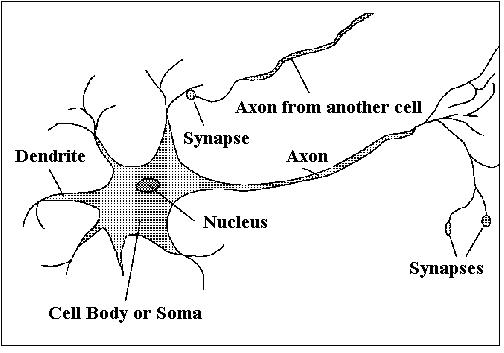
\includegraphics[width=300pt,height=200pt,scale=2]{Pics/neuron.jpg}
\centering
\caption{A neuron}
\end{figure}

One of the most important parts of the neuron structure is the synapse. The synapse is the contact between the axon of a neuron and the dendrite or the soma of another. It is where a information from one neuron is transmitted to the other. When a set of neurons are connected with each other through synapses, then they create a neural network.

Finally, the communication between neurons is accomplihed through spikes, which are either chemichal or electrical\cite{gerstner2002spiking}.

Given the terms in this section, the name of the SpiNNaker chip is detuctable. It stands for Spi(king)N(eural)N(etwork) architecture.
\subsection{The SpiNNaker architecture}
\subsection{The Conjugate Gradient Method}
The conjugate gradient method is an algorithm for the numerical solution of systems of linear eqations of the type Ax=b, those whose matrix is symmetric and positive definite. 

A \emph{symmetric} matrix is a matrix which is equal to its transpose. If A is a symmetric matrix then A=A$^T$. The entries of the matrix are symmetric with respect to the main diagonal, so if an element of the matrix A is a, then a$_{ij}$=a$_{ji}$. 
A \emph{positive definite} matrix M is a matrix which when multipled by any non-zero vector z and its transpose z$^T$, is always positive. In short the relationship that needs to be satisfied is zMz$^T$>0

It is an iterative method, which means it can be applied to sparse systems. A \emph{sparse matrix} is a matrix which is populated primirily with zeros. Its opposite would be a \emph{dense matrix}. It was developed by Magnus Hestenes and Eduard Stiefel and can be used to solve optimization problems\cite{press2007numerical}.
\subsubsection{The quadratic form}
In order to explain why the Conjugate Gradient Method can solve problems whose matrix is positive-definite and symmetric an explanation of the quadratic form needs to be presented.
\begin{center}
\begin{equation}
f(x)=\frac{1}{2}x^TAx-b^T+c
\end{equation}
\end{center}

The gradient $\nabla f(x)$ of the quadratic form is a vector field that points in the direction of the greatest increase of $f(x)$. If we were to take into account the i$^{th}$ component of $\nabla f$, then.
\begin{equation}
\begin{split}
f(x+\psi e_i)= \frac{1}{2} (x+\psi e_i)^TA(x+\psi e_i)-b^T(x+\psi e_i)+c\\
= \frac{1}{2} (x^TAx+\psi e^T_iAx +x^TA\psi e_i)-b^T(x+\psi e_i)+c
\end{split}
\end{equation}
Note that e$_i$ is the error affiliated with taking the i$^{th}$ component of $\nabla f$. Now from the definition of a derivative $f(x)$=$\frac{f(a+h)-f(a)}{h}$ and (2) we have.
\begin{equation}
\frac{f(x+\psi e_i)-f(x)}{\psi}=\frac{\frac{1}{2}(\psi e^T_iAx+x^TA\psi e_i)-\psi e^T_ib}{\psi}
\end{equation}
(3) is the same as the i$^{th}$ component of $\frac{1}{2}$(Ax+A$^T$x)-b
So we have
\begin{equation}
\nabla f =\frac{1}{2}A^Tx+\frac{1}{2}Ax-b
\end{equation}
But if A is symmetric, then it is obvious that we have $Ax=b$ at the minimum of $f$. In addition if A is positive negative then $f$ is concave up.
\subsubsection{Conjugate Gradients}
As mentioned before the matrix A must be symmetric and positive definite for the Conjugate Gradient Method to work. Given a quadratic function 
as defined in (1), then it turns out that $-\nabla f=b-Ax=r$.

The CGM as well as most optimization methods look towards a specifin direction everytime they are to move to a correct position and try to look for the best step given their gradient and direction
\begin{equation}
x_{k+1} = x_k + \alpha p_k
\end{equation}
Given (5), $\alpha$ also needs to be chosen so that $f(x_k+\alpha p_k)$ is minimized in the direction of $p_k$
\begin{equation}
0=\frac{d}{d\alpha}f(x_{k+1})=\nabla f(x_{k+1})^T\frac{d}{d\alpha}x_{k+1} = -r^T_{k+1}\frac{d}{d\alpha}(x_k + \alpha p_k) = -r^T_{k+1}p_k
\end{equation}

As it is for the method of the Steepest Descent, $\alpha$ should be set in a way that $f$ is minimized in the direction $\nabla f=r$
\begin{equation}
0=\frac{d}{d\alpha}f(x_{k+1})=\nabla f(x_{k+1})^T\frac{d}{d\alpha}x_{k+1} = -r^T_{k+1}\frac{d}{d\alpha}(x_k + \alpha r_k) = -r^T_{k+1}r_k
\end{equation}
We need to pick $\alpha$ so that $\nabla f(x_{k+1})$ and r$_k$ are orthogonal. But since we have that $\nabla f(x_{k+1})$=-r$_{k+1}$ then

\begin{equation}
\begin{split}
r^T_{k+1}r_k=0\\
(b-A(x_k+\alpha r_k)^T)r_k=0\\
(b-Ax_k)^Tr_k-\alpha(Ar_k)^Tr_k=0\\
r^T_kr_k=\alpha r^T_kAr_k\\
\alpha=-\frac{r^T_kr_k}{r^T_kAr_k}
\end{split}
\end{equation}
(8) gives the optimal value for $\alpha$.
\subsubsection{The algorithm}
Combining the optimal value of $\alpha$(8) and a good step direction for p$_k$ the Conjugate Gradient Method is formed as follows
\\
\begin{algorithmic}
\STATE r$_0$=b-Ax$_0$
\STATE p$_0$=r$_0$
\STATE k=0
\FOR{k to 1000000}
\STATE $alpha_k=\frac{r_k ^T*r_k}{p_k ^T*A*p_k}$
\STATE x$_{k+1}$=x$_k$+alpha$_k$*p$_k$
\STATE r$_{k+1}$=r$_k$-alpha$_k$*p$_k$*A
\IF{r$_{k+1}^T$*r$_{k+1}$ is small enough}
\STATE break
\ENDIF
\STATE $beta_k=\frac{r_{k+1} ^T*r_{k+1}}{r_k ^T*r_k}$
\STATE r$_{k+1}$=r$_{k+1}$+beta$_k$*p$_k$
\STATE k=k+1
\ENDFOR
\end{algorithmic}
\vspace{20pt}
Some notes that can be made about this algorithm are that the axis is defined by the eigenvectors of A and that the algorithm takes a conjugate step closest to $r$. Finally, the algorithm guarantees convergeance in at most n steps.\cite{press2007numerical}\cite{shewchuk1994introduction}\cite{cgm2009lec}

Ofcourse there is an error that exists in every step, as mentioned before, but it is minimized in each iteration. The error function would be:
\begin{equation}
\begin{vmatrix}
e_k
\end{vmatrix}
\leq 2(\frac{\sqrt{\kappa}-1}{\sqrt{\kappa}+1})^k
\begin{vmatrix}
e_0
\end{vmatrix}_A
\end{equation}

In Equation 9 $\kappa$ is the condition number.

Another interesting applicatoin of the Conjugate Gradient Method is that you can apply precondition on it in order to find the solution faster. However, preconditioning is outside of the scope of this project, since it adds a lot more calculation and would need a less general solution.
\subsubsection{Parallel solutions of the CGM}

Some parallel implementations of the CGM use blocks of the input vectors and matrix and assign them carefully to specific cores, thus letting each core produce output that will be used in the next iteration. These kinds of solutions work better with vector processors, since it allows a processor to complete large vector operations. Depending on how many processors a machine has, parts of the algorithm can continue being sliced to blocks, until the optimal implementation is reached\cite{o1987parallel}.

Some other parallel implementations try to use more specific preconditionings to achieve faster results, but again for the parallel part, they split the input into blocks to distribute it to various cores\cite{adams1985m}\cite{adams1983m}. 

One of the most interesting implementations of the CGM, suggests an improved algorithm named ICGS(Improved Conjugate Gradient Squared), which is based in another already altered version of the CGM\cite{maheswaran1999mcgs}. This implementation computes all vector-matrix  multiplications and inner products concurrently, for each iteration. The communication time between these operations and vector updates has been organised efficiently, so that global communication drops significantly, thus dropping the run time of the algorithm as well\cite{yang2001improved}.

Finally, there are many recent implementations which have used GPU's in order to solve the Conjugate Gradient Method efficiently. These pieces of work use CUDA and various other techniques to accomplish their goal, with some very good results. Ofcourse different GPU models are used, but that just enhances the generality of the solution. Generally though,as is for most parallel implementations of the CGM, the most used technique is reducing the time it takes to compute the matrix-vector multiplication and inner products, thus reducing the time of the algorithm overall\cite{galiano2012gpu}\cite{wozniak2010parallel}.
\newpage
\bibliographystyle{plain}
\bibliography{ref.bib}
\cite{navaridas2009understanding}
\cite{sharp2012power}
\cite{davies2010interfacing}
\cite{sharp2011event}
\cite{gerstner2002spiking}
\cite{press2007numerical}
\cite{shewchuk1994introduction}
\cite{cgm2009lec}
\cite{o1987parallel}
\cite{adams1985m}
\cite{maheswaran1999mcgs}
\cite{yang2001improved}
\cite{adams1983m}
\cite{galiano2012gpu}
\cite{wozniak2010parallel}
\cite{hestenes1952methods}
\end{document}